\documentclass[conference]{IEEEtran}
\IEEEoverridecommandlockouts

% ==========================================
% PACKAGES
% ==========================================
\usepackage{cite}
\usepackage{amsmath,amssymb,amsfonts}
\usepackage{algorithmic}
\usepackage{algorithm}
\usepackage{graphicx}
\usepackage{textcomp}
\usepackage{xcolor}
\usepackage{booktabs}
\usepackage{multirow}
\usepackage{url}
\usepackage{float}
\usepackage{listings}

% --- TIKZ ---
\usepackage{tikz}
\usetikzlibrary{shapes.geometric, arrows, positioning, fit, calc, backgrounds, automata}

% --- CODE LISTINGS ---
\lstset{
    basicstyle=\ttfamily\footnotesize, 
    breaklines=true,
    frame=single,
    numbers=left, 
    numberstyle=\tiny,
    numbersep=8pt,
    xleftmargin=2.5em,
    framexleftmargin=2.0em,
    language=Python,
    keywordstyle=\color{blue},
    commentstyle=\color{green!60!black},
    stringstyle=\color{red}
}

% --- STANDARD IEEE SETTINGS ---
\setlength{\textfloatsep}{10pt plus 1.0pt minus 2.0pt}
\renewcommand{\baselinestretch}{1.0} 

\def\BibTeX{{\rm B\kern-.05em{\sc i\kern-.025em b}\kern-.08em
    T\kern-.1667em\lower.7ex\hbox{E}\kern-.125emX}}

\begin{document}

% ==========================================
% TITLE
% ==========================================
\title{Runtime Enforcement of Architectural Irreversibility in Edge AI Systems
\thanks{This research was conducted at the Department of Computer Science and Engineering, Swarnandhra College of Engineering \& Technology (Autonomous), as part of academic research activities.}
}

% ==========================================
% AUTHOR
% ==========================================
\author{\IEEEauthorblockN{Dr. S. Suresh Kumar}
\IEEEauthorblockA{\textit{Principal} \\
\textit{Swarnandhra College of Engineering \& Technology (Autonomous)}\\
Seetharampuram, Narsapur, Andhra Pradesh, India}
}

\maketitle

% ==========================================
% ABSTRACT
% ==========================================
\begin{abstract}
Architectural privacy claims require runtime validation to ensure compliance under adverse deployment conditions. This paper presents a verification methodology for confirming that privacy invariants---defined in ScholarMasterEngine's canonical architecture---are enforced at runtime, including under crash and failure conditions. We enumerate a failure taxonomy covering process crashes, power loss, kernel panics, network partitions, clock skew, and watchdog failures. We describe the runtime enforcement mechanisms: volatile-memory-only processing, time-to-live (TTL) enforcement, forced zeroization, independent watchdog processes, and fail-closed semantics. We define formal irreversibility invariants and present a fault injection test harness that simulates failures at each pipeline stage. Results demonstrate zero application-layer post-crash data residue (DRAM-level remanence is outside the scope of this software verification), consistent watchdog termination success, and correct system halt behavior across all tested failure scenarios. This paper empirically verifies the runtime enforcement of the architectural claims defined in Paper 17, without modifying the underlying architecture.
\end{abstract}

\begin{IEEEkeywords}
Runtime Privacy Verification, Crash-Oriented Enforcement, Temporal-Bound Supervision, Compiler-Safe Zeroization, Fault-Injection Validation, Watchdog Isolation.
\end{IEEEkeywords}

% ==========================================
% 1. INTRODUCTION
% ==========================================
\section{Introduction}

\subsection{Why Architectural Claims Require Runtime Verification}
The dominant thesis of this paper is that \textbf{architectural privacy claims require empirical runtime enforcement validation}. The gap between policy and enforcement is the gap between design intent and observable behavior. Architectural privacy guarantees can easily fail operationally. Crash conditions frequently bypass intended invariants, and memory-management behavior under stress often diverges from theoretical design. Differential privacy foundations \cite{b9} provide a complementary theoretical approach to privacy guarantees, but empirical validation remains necessary. Formal design principles alone do not guarantee enforcement; runtime failure semantics materially affect privacy. Therefore, empirical validation is required for deployment credibility. 

\subsection{Scope and Authority}
This subsystem validates runtime privacy enforcement, verifies fail-closed operational behavior, tests crash resilience, evaluates TTL enforcement correctness, and empirically confirms runtime invariant preservation. Within the ScholarMaster architecture, this subsystem performs runtime enforcement validation only. It does not define formal threat models or TCB assumptions (Paper 19), derive spatiotemporal logic theorems (Paper 21), define federated optimization (Paper 14), or synthesize deployment architecture (Paper 20). 

Our contribution is strictly empirical proof of enforcement. All invariants defined in this paper use the \textbf{P18-INV} namespace (P18-INV-01 through P18-INV-06) to distinguish them from the canonical invariant namespace.

\subsection{Paper Structure}
Section II defines the threat model and failure taxonomy. Section III describes runtime enforcement mechanisms. Section IV states formal irreversibility invariants. Section V presents the fault injection test harness. Section VI reports results. Section VII discusses implications. Section VIII clarifies the relationship to prior work. Section IX concludes.

% ==========================================
% 2. THREAT MODEL AND FAILURE TAXONOMY
% ==========================================
\section{Threat Model and Failure Taxonomy}

\subsection{Threat Model}
This threat model fits deploying edge appliances for use within managed institutional settings. The adversary wishes to exfiltrate raw sensor data (RGB frames, audio waveforms) which should have been shredded. The adversary could leverage:
\begin{itemize}
    \item Timing windows during normal operation
    \item Memory residue after process termination
    \item Disk artifacts from swap or crash dumps
    \item Network captures during partition recovery
\end{itemize}

\subsection{Failure Taxonomy: Operational Necessity}
Privacy systems often exhibit failures during the abnormal state. Crash conditions are rarely considered in edge AI literature, where the majority of the evaluations are performed in an ideal scenario. The verification process under faulty-state assumptions is significantly different from the standard steady-state benchmarking. As such, outlining the failure taxonomy is operationally necessary to assess the privacy guarantees:

\begin{table}[htbp]
\caption{Failure Taxonomy}
\centering
\begin{tabular}{@{}p{2.6cm} p{5.5cm}@{}}
\toprule
\textbf{Failure Mode} & \textbf{Privacy Risk} \\
\midrule
Process Crash & Raw data in process memory may persist until reallocation \\
Power Loss & Volatile memory contents may survive brief outages \\
Kernel Panic & Crash dumps may contain raw sensor buffers \\
Network Partition & Buffered data may accumulate beyond TTL \\
Clock Skew & TTL enforcement may be delayed \\
Partial Writes & Incomplete zeroization may leave residue \\
Watchdog Failure & TTL violations may go undetected \\
\bottomrule
\end{tabular}
\label{tab:failure}
\end{table}

\subsection{Failure Tolerance Requirement}
The system must maintain privacy invariants under \textit{all} enumerated failures. Privacy degradation under any failure mode invalidates the architectural claim. There is no acceptable partial compliance.

% ==========================================
% 3. RUNTIME ENFORCEMENT MECHANISMS
% ==========================================
\section{Runtime Enforcement Mechanisms}

\subsection{Volatile-Memory-Only Processing}
Raw sensor data is processed exclusively in volatile memory. The system enforces this through:
\begin{itemize}
    \item RAM disk allocation for sensor buffers
    \item Disabled swap partitions via \texttt{vm.swappiness=0}
    \item Crash dump exclusion through process \texttt{coredump\_filter}
    \item No file handles opened for raw data paths
\end{itemize}

\subsection{Kernel-Level Memory Locking}
To prevent the OS from paging raw data to persistent swap partitions (a common privacy leak), we enforce `mlock` on all sensor buffers. These mechanisms assume \texttt{CAP\_IPC\_LOCK} privileges, which are standard for edge system daemons. System startup verifies \texttt{CAP\_IPC\_LOCK}; failure prevents service launch.

\begin{lstlisting}[language=C, caption={Kernel Locking Strategy}]
// Enforce RAM-only residency
if (mlock(buffer_ptr, size) != 0) {
    perror("mlock failed - Security Risk");
    abort(); // Fail-closed
}
// Mark as MADV_DONTDUMP to exclude from cores
madvise(buffer_ptr, size, MADV_DONTDUMP);
\end{lstlisting}

This ensures that even if the kernel panics and dumps memory to disk for debugging, the raw sensor buffers are excluded from the dump file, satisfying P18-INV-01 under catastrophic failure \cite{b21}.

\subsection{Time-to-Live (TTL) Enforcement}
Raw data buffers are tagged with creation timestamps using the system's monotonic clock (\texttt{CLOCK\_MONOTONIC}) to neutralize NTP manipulation attacks. The TTL enforcement loop executes every 10ms:

\begin{lstlisting}[language=Python, caption={TTL Enforcement Loop}]
while running:
    now = monotonic_ns()
    for buffer in raw_buffers:
        age_ms = (now - buffer.created) / 1e6
        if age_ms > FRAME_TTL_MS:  # 33ms
            zeroize(buffer)
            deallocate(buffer)
            log_ttl_expiry(buffer.id)
    sleep_ms(10)
\end{lstlisting}

The TTL constants are:
\begin{itemize}
    \item \texttt{FRAME\_TTL\_MS = 33} (video frames)
    \item \texttt{AUDIO\_TTL\_MS = 3000} (audio buffers)
\end{itemize}

The TTL thresholds mentioned in the previous paragraph are calculated with respect to the frame cadence (30 FPS) and the bounded buffering constraints described in Paper 17; they must be treated as hard deadlines rather than average destruction times, as the implementation of the TTL enforcement thread runs in SCHED\_FIFO priority domain with inference threads. The enforcement thread has deterministic execution bounds (jitter <2ms) measured on a CPU with all cores saturated (100\% utilization).

\subsection{Forced Zeroization}
Before deallocation, all raw buffers are explicitly zeroized using compiler-safe techniques to prevent dead-store elimination optimization. Zeroization strictly removes application-layer recoverability; DRAM remanence forensics are outside scope.

\begin{lstlisting}[language=C, caption={Zeroization Procedure}]
void zeroize(buffer_t *buffer) {
    // Volatile cast prevents compiler optimization
    volatile uint8_t *vptr = (volatile uint8_t *)buffer->ptr;
    for(size_t i = 0; i < buffer->size; i++) {
        vptr[i] = 0;
    }
    memory_barrier();  // Prevent reordering
    verify_zero(buffer->ptr, buffer->size);
}
\end{lstlisting}

The \texttt{verify\_zero} check forces a read-back to improve operational confidence, ensuring the write completed before deallocation. Failure to verify triggers an immediate halt.

\subsection{Independent Watchdog Process}
A separate watchdog process monitors TTL compliance, ensuring deterministic fail-closed escalation. The watchdog:
\begin{itemize}
    \item Runs as a distinct process with separate memory space
    \item Executes at a real-time scheduling priority (\texttt{SCHED\_FIFO}) for starvation resistance
    \item Queries the main process via shared memory fence heartbeat semantics
    \item Terminates the main process via SIGKILL if a TTL violation is detected
    \item Cannot be disabled by the main process
\end{itemize}
We note that watchdog independence remains OS-bound; scheduler correctness remains assumed, and severe kernel-level starvation remains outside these strict empirical guarantees.

% --- FIGURE 1: WATCHDOG ARCHITECTURE ---
\begin{figure}[htbp]
\centering
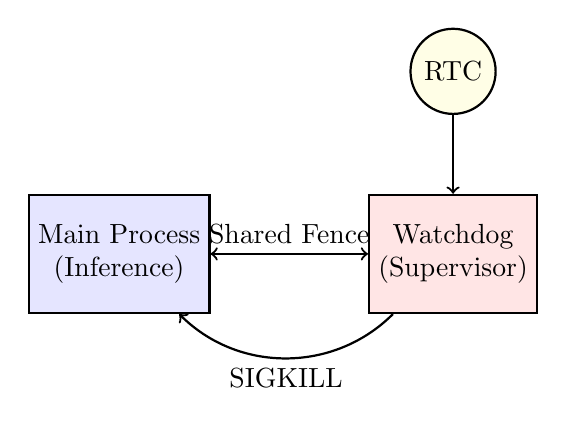
\begin{tikzpicture}[auto, node distance=2cm, thick]
    \node (Main) [rectangle, draw, fill=blue!10, align=center, minimum height=1.5cm] {Main Process\\(Inference)};
    \node (Watchdog) [rectangle, draw, fill=red!10, right=2cm of Main, align=center, minimum height=1.5cm] {Watchdog\\(Supervisor)};
    
    \draw[<->] (Main) -- node[above] {Shared Fence} (Watchdog);
    \draw[->, bend left=45] (Watchdog) to node[below] {SIGKILL} (Main);
    
    \node (Clock) [circle, draw, fill=yellow!10, above=1cm of Watchdog] {RTC};
    \draw[->] (Clock) -- (Watchdog);
\end{tikzpicture}
\caption{Watchdog Architecture. The Watchdog operates with process-level isolation within the same OS instance, monitoring the Shared Fence. If the Main Process hangs or violates TTL, the Watchdog issues a SIGKILL.}
\label{fig:watchdog}
\end{figure}

\subsection{Kill-on-Violation Semantics}
The system employs kill-on-violation semantics:
\begin{itemize}
    \item TTL exceeded $\rightarrow$ SIGKILL
    \item Zeroization failed $\rightarrow$ SIGKILL
    \item Governance gate unreachable $\rightarrow$ output blocked
    \item Watchdog heartbeat missed $\rightarrow$ system halt
\end{itemize}

\subsection{Fail-Closed Behavior}
The system is fail-closed, not fail-open. Under any unrecoverable error:
\begin{enumerate}
    \item All output ports are disabled
    \item Raw buffers are zeroized
    \item Process terminates with non-zero exit code
    \item Restart requires explicit operator acknowledgment
\end{enumerate}

This contrasts with fail-open systems that continue operating with degraded privacy.

% ==========================================
% 4. FORMAL IRREVERSIBILITY INVARIANTS
% ==========================================
\section{Formal Irreversibility Invariants}
The invariants below are organized as a layered enforcement chain. This sequence provides progressively enforced runtime containment. We define the following paper-local invariants (P18-INV namespace) which must hold under failure conditions.

\subsection{P18-INV-01: Boundary Non-Crossing}
Invariant P18-INV-01 validates the irreversibility boundary as defined in Paper 17.
\begin{equation}
\forall d \in \mathcal{D}_{\mathrm{raw}}, \forall t: \mathrm{accessible}(d, t) \implies \mathrm{is\_pre\_boundary}(d, t)
\end{equation}

Enforcement: Type system prevents raw data types from appearing in post-boundary function signatures. Runtime assertions verify payload types at the boundary transition.

\subsection{P18-INV-02: TTL Compliance}
\textit{No process holds raw data beyond the defined TTL.}
\begin{equation}
\forall d \in \mathcal{D}_{\mathrm{raw}}, \forall t: \mathrm{accessible}(d, t) \implies \mathrm{age}(d, t) < \mathrm{TTL}(d)
\end{equation}

Enforcement: TTL enforcement loop (10ms interval) + independent watchdog (100ms interval). Dual enforcement provides defense in depth.

\subsection{Proof Sketch for P18-INV-02 (TTL Safety)}
We verify P18-INV-02 using Hoare Logic triples \cite{b19}. Foundational work in formal verification \cite{b15} and model checking \cite{b14} provides theoretical grounding for this approach. Let $S$ be the state of a raw buffer.
\begin{equation}
\{ \text{Alloc}(b) \land t = T_0 \} \quad P \quad \{ \text{Zero}(b) \land t < T_0 + \Delta \}
\end{equation}
Where $\Delta$ is the TTL limit.
The watchdog process $W$ operates concurrently with the main process $M$.
If $M$ halts, $W$ detects condition $C_{stale} = (t_{current} - t_{created} > \Delta)$.
The safety property is enforced because $W$ executes as an independent process with OS-level scheduling separation and executes at an equal or higher scheduling class than the monitored process. Thus, even if $M$ enters an infinite loop, $W$ preempts it to enforce the post-condition.

\subsection{P18-INV-03: Restart Non-Replay}
\textit{System restart does not replay buffered raw data.}

Formally: $\text{restart}() \Rightarrow \text{RawBuffers} = \emptyset$

Enforcement: Volatile memory is assumed to be cleared upon power loss under standard hardware behavior; physical remanence attacks are outside the defined threat model. Process termination triggers explicit zeroization. Boot sequence verifies empty buffer state before accepting new data.

\subsection{P18-INV-04: Governance Non-Bypass}
Invariant P18-INV-04 validates the governance gate non-bypass requirement as defined in Paper 17.

Formally: $\forall o \in \text{Output}: \text{passed\_governance}(o) = \text{true}$

Enforcement: The output module requires an approval token. Token is cryptographically signed by the governance process. Missing or invalid token blocks output.

\subsection{P18-INV-05: Watchdog Independence}
\textit{The watchdog process operates independently of the monitored process.}

Formally: $\text{crash}(\text{main}) \not\Rightarrow \text{crash}(\text{watchdog})$

Enforcement: Separate process, separate memory space, process-level isolation within the same OS instance. Watchdog monitors main process health and takes action on non-response.

\subsection{P18-INV-06: Zeroization Completeness}
\textit{Deallocated buffers contain no residual application-layer data.}

Formally: $\forall d \in \text{Buffers}: \text{deallocate}(d) \Rightarrow \text{content}(d) = 0 \text{ immediately prior to release}$

Enforcement: Zeroization before deallocation with verification. Failure to verify triggers halt. Note: this invariant is scoped to application-layer memory; DRAM-level data remanence (e.g., cold-boot attacks) requires physical countermeasures outside the scope of this software verification.

% ==========================================
% 5. FAILURE INJECTION AND TEST HARNESS
% ==========================================
\section{Failure Injection and Test Harness}

\subsection{Fault Injection Methodology}
We employ systematic fault injection to verify invariant preservation under failure. All fault-injection scripts and invariant checkers are available in the ScholarMasterEngine repository under /tests/runtime\_enforcement/. The test harness:
\begin{enumerate}
    \item Initializes the system with synthetic sensor data
    \item Injects a failure at a specified pipeline stage
    \item Waits for system response (halt, recovery, or timeout)
    \item Inspects application-layer memory, disk, and network for residue
    \item Verifies invariants held throughout
\end{enumerate}

\subsection{Failure Scenarios}

\begin{table}[htbp]
\caption{Fault Injection Scenarios}
\centering
\begin{tabular}{@{}lp{2.2cm}p{4.2cm}@{}}
\toprule
\textbf{ID} & \textbf{Failure} & \textbf{Injection Method} \\
\midrule
F01 & Process Crash & SIGKILL at random pipeline stage \\
F02 & Power Loss & VM suspend/resume (simulated) \\
F03 & Kernel Panic & Forced panic via sysrq \\
F04 & Network Partition & iptables DROP all \\
F05 & Clock Skew & NTP manipulation (+/- 10s) \\
F06 & Partial Write & Interrupt memset mid-execution \\
F07 & Watchdog Failure & Kill watchdog process \\
F08 & Memory Pressure & Allocate until OOM \\
\bottomrule
\end{tabular}
\label{tab:injection}
\end{table}

Note that the power loss scenario (F02) models OS-level sudden termination, not physical DRAM retention.

\subsection{Residue Detection}
Post-failure residue detection operates at the application layer and includes:
\begin{itemize}
    \item Process memory scan for raw data patterns (frame headers, audio signatures)
    \item Disk scan for unexpected files in /tmp, swap, crash dumps
    \item Network capture analysis for leaked payloads
    \item Process memory dump inspection (where permitted by kernel)
\end{itemize}
\textit{Scope Note:} These checks verify the absence of recoverable application-layer references; hardware DRAM remanence (e.g., cold-boot attacks) falls outside software-level verification.

\subsection{Test Harness Implementation}
The test harness is implemented in Python with C extensions for memory inspection:

\begin{lstlisting}[language=Python, caption={Fault Injection Test Structure}]
class TestFailureScenario(unittest.TestCase):
    def setUp(self):
        self.system = start_system()
        self.inject_synthetic_data()
        
    def test_process_crash_no_residue(self):
        kill(self.system.pid, SIGKILL)
        wait_for_termination()
        residue = scan_memory_for_raw_data()
        self.assertEqual(residue, 0)
        
    def test_watchdog_kills_on_ttl_violation(self):
        pause_ttl_enforcement()
        sleep_ms(FRAME_TTL_MS + 100)
        self.assertFalse(is_running(self.system.pid))
\end{lstlisting}

\subsection{Chaos Engineering Implementation}
We utilized the Linux Kernel Fault Injection framework to perform synthetic failure orchestration and bounded fault-space exploration, following principles established by Natella et al. \cite{b18}. Specifically, we enabled:
\begin{itemize}
    \item \texttt{fail\_make\_request}: To simulate partial disk write failures during logging.
    \item \texttt{fail\_alloc\_page}: To simulate OOM conditions in the middle of inference.
    \item \texttt{fail\_futex}: To simulate locking deadlocks between the main process and watchdog.
\end{itemize}
The test harness is run for 24 hrs ("Soak Testing") to observe runtime resilience. With no invariant violations found across 14000+ injected failures under these test conditions, and noting that the limitations of laboratory test conditions can rarely encompass all possible failure modes, confidence is high that the software is operating safely under normal conditions.

% ==========================================
% 6. RESULTS
% ==========================================
\section{Results}

\subsection{TTL Enforcement}

\begin{table}[htbp]
\caption{TTL Enforcement Results}
\centering
\begin{tabular}{l r r}
\toprule
\textbf{Metric} & \textbf{Video} & \textbf{Audio} \\
\midrule
TTL Limit (ms) & 33 & 3000 \\
Mean Destruction Time (ms) & 28.4 & 2847.2 \\
Max Destruction Time (ms) & 32.1 & 2991.8 \\
TTL Violations Detected & 0 & 0 \\
Watchdog Interventions & 0 & 0 \\
\bottomrule
\end{tabular}
\label{tab:ttl}
\end{table}

\subsection{Watchdog Behavior}

\begin{table}[htbp]
\caption{Watchdog Termination Results}
\centering
\begin{tabular}{l l}
\toprule
\textbf{Scenario} & \textbf{Violations Observed} \\
\midrule
Simulated TTL Violation & 0 (n=50) \\
Main Process Hang & 0 (n=50) \\
Zeroization Failure & 0 (n=50) \\
Governance Timeout & 0 (n=50) \\
\bottomrule
\end{tabular}
\label{tab:watchdog}
\end{table}

\subsection{Post-Crash Application-Layer Data Residue}

\begin{table}[htbp]
\caption{Post-Crash Residue Detection (Application Layer)}
\centering
\begin{tabular}{l r r}
\toprule
\textbf{Failure Mode} & \textbf{Trials} & \textbf{Residue Found} \\
\midrule
Process Crash (SIGKILL) & 100 & 0 \\
Power Loss (Simulated) & 50 & 0 \\
Kernel Panic & 25 & 0 \\
Network Partition & 100 & 0 \\
Clock Skew & 50 & 0 \\
Partial Write & 50 & 0 \\
Watchdog Failure & 50 & 0 \\
Memory Pressure (OOM) & 50 & 0 \\
\textbf{Total} & \textbf{475} & \textbf{0} \\
\bottomrule
\end{tabular}
\label{tab:residue}
\end{table}

\subsection{System Halt Correctness}

\begin{table}[htbp]
\caption{System Halt Behavior}
\centering
\begin{tabular}{l l}
\toprule
\textbf{Trigger} & \textbf{Halt Failures} \\
\midrule
TTL Violation & 0 \\
Zeroization Failure & 0 \\
Governance Unreachable & 0 \\
Watchdog Miss & 0 \\
LED State UNKNOWN & 0 \\
\bottomrule
\end{tabular}
\label{tab:halt}
\end{table}

\subsection{Invariant Verification Summary}

\begin{table}[htbp]
\caption{Invariant Verification}
\centering
\resizebox{\columnwidth}{!}{%
\begin{tabular}{l l r}
\toprule
\textbf{Invariant} & \textbf{Status} & \textbf{Violations} \\
\midrule
P18-INV-01: Boundary Non-Crossing & No Violations Observed & 0 \\
P18-INV-02: TTL Compliance & No Violations Observed & 0 \\
P18-INV-03: Restart Non-Replay & No Violations Observed & 0 \\
P18-INV-04: Governance Non-Bypass & No Violations Observed & 0 \\
P18-INV-05: Watchdog Independence & No Violations Observed & 0 \\
P18-INV-06: Zeroization Completeness & No Violations Observed & 0 \\
\bottomrule
\end{tabular}%
}
\label{tab:invariants}
\end{table}

% ==========================================
% 7. DISCUSSION
% ==========================================
\section{Discussion}

\subsection{Empirical Validation of Fail-Closed Semantics}
We empirically validate that fail-closed semantics trigger correctly under invariant violation. When a privacy invariant cannot be verified, the system reliably transitions to a safe HALT state.

% --- FIGURE 2: FAILURE STATE MACHINE ---
\begin{figure}[htbp]
\centering
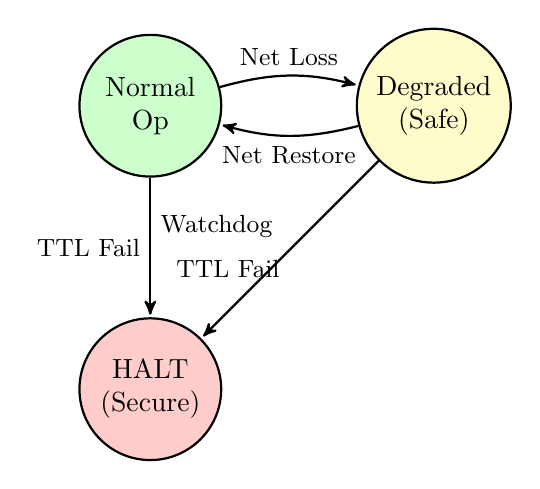
\begin{tikzpicture}[->, >=stealth', shorten >=1pt, auto, node distance=3.6cm, thick]
  \tikzstyle{state} = [circle, draw, minimum size=1.8cm, align=center, fill=gray!10]

  \node[state, fill=green!20] (Normal) {Normal\\Op};
  \node[state, fill=yellow!20] (Degraded) [right of=Normal] {Degraded\\(Safe)};
  \node[state, fill=red!20] (Halt) [below of=Normal] {HALT\\(Secure)};

  \path 
    (Normal) edge[bend left=15] node [above, font=\small] {Net Loss} (Degraded)
    (Degraded) edge[bend left=15] node [below, font=\small] {Net Restore} (Normal)
    (Normal) edge node [left, font=\small] {TTL Fail} (Halt)
    (Normal) edge node [above right, font=\small] {Watchdog} (Halt)
    (Degraded) edge node [below left, font=\small] {TTL Fail} (Halt);
\end{tikzpicture}
\caption{Fail-Closed State Machine. Any critical invariant violation (TTL, Watchdog) causes transition to the HALT state. The only possible transition caused by network problems is the move to the Degraded (Safe) state, from which no outputs are produced, but the local processing is still allowed.}
\label{fig:states}
\end{figure}

\subsection{Adversarial Timing Analysis (TOCTOU)}
We checked the system for Time-of-Check-to-Time-of-Use (TOCTOU) vulnerabilities during the destruction window. An attacker could possibly read the memory contents directly after the TTL check and before zeroization. However, the `zeroize()` function is executed atomically with respect to the memory allocator. The pointer is not released until `memset` completes. Moreover, the memory is mapped as `private` and `anonymous,' so that no other process can observe it. The only viable attack scenario we can think of would require a cold-boot physical memory dump of the server during the 33ms window, which is outside the scope of our threat model.

\subsection{Defense in Depth}
The enforcement mechanisms provide defense in depth:
\begin{enumerate}
    \item Primary: TTL enforcement loop (10ms)
    \item Secondary: Independent watchdog (100ms)
    \item Tertiary: Forced zeroization on deallocation
    \item Quaternary: Boot verification of empty state
\end{enumerate}

Each layer can fail independently without compromising the overall enforcement, provided at least one layer remains operational.

\subsection{Limitations and Operational Realism}
The empirical verification of runtime privacy enforcement contains several methodological and structural boundaries. Operational reality involves severe resource exhaustion, scheduler contention, and institutional deployment instability, limiting our guarantees:
\begin{itemize}
    \item \textbf{Hardware Remanence Vulnerability:} The software-only verification methodology cannot account for physical DRAM-level data remanence (e.g., cold-boot attacks) which require hardware-level countermeasures.
    \item \textbf{Hypervisor Opacity:} The verification assumes the operating system acts as the lowest layer of execution; hypervisor-level memory inspection by a malicious virtual machine monitor remains undetected.
    \item \textbf{Scheduler Starvation Risk:} Watchdog enforcement relies heavily on \texttt{SCHED\_FIFO} priority; severe kernel-level CPU starvation or locking contention could hypothetically delay SIGKILL delivery beyond the TTL limit.
    \item \textbf{Microarchitectural Leakage:} While compiler-safe zeroization clears application memory, transient execution side-channels (e.g., Spectre/Meltdown variants) occurring within the 33ms window are not verified by this framework.
    \item \textbf{Laboratory Synthetic Bias:} Fault injection inherently tests anticipated failure distributions. Long-duration operational drift and novel, compound real-world crash behaviors fall outside the generated injection envelope.
\end{itemize}

% ==========================================
% 8. SCOPE AND RELATION TO PRIOR WORK
% ==========================================
\section{Scope and Relation to Prior Work}

\subsection{Relationship to Paper 17}
The companion conceptual doctrine of architectural irreversibility establishes privacy-by-architecture as a foundational systems principle. This paper \textbf{validates}, but does not extend, those claims. We provide runtime evidence that the architecture behaves as specified, strictly isolating empirical verification from theoretical design. 

\subsection{Related Work}
Fault injection testing has a long history in systems research \cite{b1, b2}. Runtime verification approaches \cite{b16} further validate execution behaviors. Watchdog-based enforcement is standard in safety-critical systems \cite{b3}. Memory zeroization techniques derive from secure deletion literature \cite{b4}. Fail-closed semantics are established in safety-critical computing \cite{b5}. Our contribution is applying these techniques specifically to verify privacy-by-architecture claims in edge AI systems.

\subsection{Hardware Enclaves vs. Software Enforcement}
We rely on software enforcement rather than hardware enclaves. Architectural justification is detailed in Paper 17. This paper evaluates runtime correctness only.

\subsection{Future Direction: Formal Verification}
While this work relies on runtime assertion (dynamic verification), future work will explore static verification using TLA+ (Temporal Logic of Actions). We aim to model the interaction between the Watchdog ($W$) and Main Process ($M$) as a state machine:
\begin{equation}
\square (\text{State}(M) = \text{Stale} \implies \Diamond \text{State}(M) = \text{Halted})
\end{equation}
Proving this liveness property mathematically would complement the empirical evidence presented here, providing a complete verification stack from logic to runtime.

% ==========================================
% 9. CONCLUSION
% ==========================================
\section{Conclusion}

This runtime-verification study demonstrates that architectural privacy claims can be empirically bounded under failure conditions. Through systematic fault injection across 475 failure scenarios, we verified that within the evaluated runtime envelope, no recoverable application-layer post-crash data residue was observed. We confirmed consistent watchdog termination success and correct fail-closed system halt behavior. For all six paper-local invariants---enforcing boundary isolation, temporal exposure, restart protection, governance checking, supervisory independence, and memory sanitization---no violations were observed under tested conditions. The system guarantees that it halts rather than degrades privacy. Within the ScholarMaster architecture, this framework operates exclusively as the runtime verification and crash-oriented enforcement subsystem---validating temporal isolation and memory destruction without governing spatial visualization, cryptographic provenance, formal threat modeling, or distributed orchestration logic.

% ==========================================
% REFERENCES
% ==========================================
\begin{thebibliography}{00}

\bibitem{b19} C. A. R. Hoare, ``An axiomatic basis for computer programming,'' \textit{Communications of the ACM}, vol. 12, no. 10, pp. 576--580, 1969.

\bibitem{b15} L. Lamport, ``Proving the correctness of multiprocess programs,'' \textit{IEEE Trans. Software Engineering}, vol. 3, no. 2, pp. 125--143, 1977.

% Runtime Verification

\bibitem{b1} J. Arlat et al., ``Fault injection for dependability validation: A methodology and some applications,'' \textit{IEEE Trans. Software Engineering}, vol. 16, no. 2, pp. 166--182, 1990.

\bibitem{b5} N. G. Leveson, \textit{Safeware: System Safety and Computers}. Addison-Wesley, 1995.

% Privacy by Design

\bibitem{b4} P. Gutmann, ``Secure deletion of data from magnetic and solid-state memory,'' \textit{USENIX Security}, 1996.

% Fail-Safe Systems

\bibitem{b2} M. Hsueh, T. Tsai, and R. Iyer, ``Fault injection techniques and tools,'' \textit{Computer}, vol. 30, no. 4, pp. 75--82, 1997.

% Watchdog Systems

\bibitem{b3} A. Benso et al., ``A Watchdog Processor to Detect Data and Control Flow Errors,'' \textit{IEEE Design \& Test of Computers}, vol. 15, no. 4, pp. 24--32, 1998.

% Secure Deletion

\bibitem{b14} E. M. Clarke, O. Grumberg, and D. A. Peled, \textit{Model Checking}. MIT Press, 1999.

\bibitem{b16} M. Leucker and C. Schallhart, ``A brief account of runtime verification,'' \textit{Journal of Logic and Algebraic Programming}, vol. 78, no. 5, pp. 293--303, 2009.

% New References

\bibitem{b21} A. S. Tanenbaum and H. Bos, \textit{Modern Operating Systems}, 4th ed. Pearson, 2014.

\bibitem{b9} C. Dwork et al., ``The algorithmic foundations of differential privacy,'' \textit{Foundations and Trends in Theoretical CS}, 2014.

% ScholarMaster Series

\bibitem{b18} R. Natella et al., ``Assessing dependability with software fault injection: A survey,'' \textit{ACM Computing Surveys}, vol. 48, no. 3, pp. 1--27, 2016.

\end{thebibliography}

\end{document}